\documentclass[a4paper, 10pt]{article}
\title{Homework}
\author{S. Schreiber}
\date{\today}
\usepackage{float}
\usepackage{tikz}
\usepackage{graphicx}
\usetikzlibrary{arrows, automata}
\begin{document}
\maketitle
\section*{Question 2.1}
\subsection*{(a)}
\subsubsection*{Parse tree}
 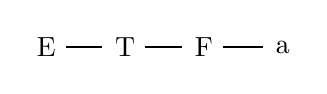
\begin{tikzpicture}[-,>=stealth',shorten >=1pt,auto,node distance=1cm,
  thick,main node/.style={circle,fill=blue!20,draw,font=\sffamily\Large\bfseries}]
  \node[] (1) {E};
  \node[] (2) [right of=1] {T};
  \node[] (3) [right of=2] {F};
  \node[] (4) [right of=3] {a};
  \path[every node/.style={font=\sffamily\small}]
    (1) edge node {} (2)
    (2) edge node {} (3)
    (3) edge node {} (4);
  \end{tikzpicture}
  \subsubsection*{Derivation}
   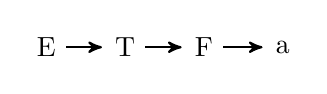
\begin{tikzpicture}[->,>=stealth',shorten >=1pt,auto,node distance=1cm,
  thick,main node/.style={circle,fill=blue!20,draw,font=\sffamily\Large\bfseries}]
  \node[] (1) {E};
  \node[] (2) [right of=1] {T};
  \node[] (3) [right of=2] {F};
  \node[] (4) [right of=3] {a};
  \path[every node/.style={font=\sffamily\small}]
    (1) edge node {} (2)
    (2) edge node {} (3)
    (3) edge node {} (4);
  \end{tikzpicture}
  \subsection*{(b)}
\subsubsection*{Parse tree}
 \begin{tikzpicture}[-,>=stealth',shorten >=1pt,auto,node distance=1cm,
  thick,main node/.style={circle,fill=blue!20,draw,font=\sffamily\Large\bfseries}]
  \node[] (h) {};
  \node[] (1) [right of=h,right of=h,right of=h] {E};
  \node[] (2) [below of=1,below of=1,below of=1,below of=1] {+};
  \node[] (3) [below of=1,left of=1] {E};
  \node[] (4) [below of=3] {T};
  \node[] (5) [below of=4] {F};
  \node[] (6) [below of=5] {a};
  \node[] (7) [below of=1,right of=1] {T};
  \node[] (8) [below of=7] {F};
  \node[] (9) [below of=8, below of=8] {a};
 
  \path[every node/.style={font=\sffamily\small}]
    (1) edge node {} (2)
    		edge [bend right] node {} (3)
    		edge [bend left]node {} (7)
    (3) edge node {} (4)
    (4) edge node {} (5)
    (5) edge node {} (6)
    (7) edge node {} (8)
    (8) edge node {} (9);
  \end{tikzpicture}
  \subsubsection*{Derivation}
   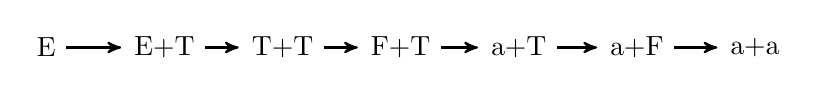
\begin{tikzpicture}[->,>=stealth',shorten >=1pt,auto,node distance=1.5cm,
  thick,main node/.style={circle,fill=blue!20,draw,font=\sffamily\Large\bfseries}]
  \node[] (1) {E};
  \node[] (2) [right of=1] {E+T};
  \node[] (3) [right of=2] {T+T};
  \node[] (4) [right of=3] {F+T};
  \node[] (5) [right of=4] {a+T};
  \node[] (6) [right of=5] {a+F};
  \node[] (7) [right of=6] {a+a};
  \path[every node/.style={font=\sffamily\small}]
    (1) edge node {} (2)
    (2) edge node {} (3)
    (3) edge node {} (4)
    (4) edge node {} (5)
    (5) edge node {} (6)
    (6) edge node {} (7);
  \end{tikzpicture}
  \subsection*{(c)}
\subsubsection*{Parse tree}
\begin{tikzpicture}[-,>=stealth',shorten >=1pt,auto,node distance=1cm,
  thick,main node/.style={circle,fill=blue!20,draw,font=\sffamily\Large\bfseries}]
  \node[] (h) {};
  \node[] (1) [right of=h,right of=h,right of=h] {E};
  \node[] (2) [below of=1] {+};
  \node[] (3) [below of=1,left of=1,left of=1] {E};
  
  %1
  \node[] (4) [below of=3,left of=3] {E};
  %2  
  \node[] (5) [below of=3] {+};
  %3  
  \node[] (6) [below of=3,right of=3] {T};

%1
 \node[] (7) [below of=4] {T};
 \node[] (8) [below of=7] {F};
 \node[] (9) [below of=8] {a};
 
 %3
 \node[] (10) [below of=6] {F};
 \node[] (11) [below of=10] {a};
 
 \node[] (12) [below of=1,right of=1,right of=1] {T};
 \node[] (13) [below of=12] {F};
 \node[] (14) [below of=13] {a};
  \path[every node/.style={font=\sffamily\small}]
    (1) edge node {} (2)
    		edge [bend right] node {} (3)
    		edge [bend left] node {} (12)
    	(3) edge[bend right] node {} (4)
    		edge node {} (5)
    		edge[bend left] node {} (6)
    	(4) edge node {}(7)
    	(7) edge node {}(8)
    	(8) edge node {}(9)
    	(6) edge node {}(10)
    	(10) edge node {}(11)
    	(12) edge node {}(13)
    	(13) edge node {}(14);
  \end{tikzpicture}
\subsubsection*{Derivation}
  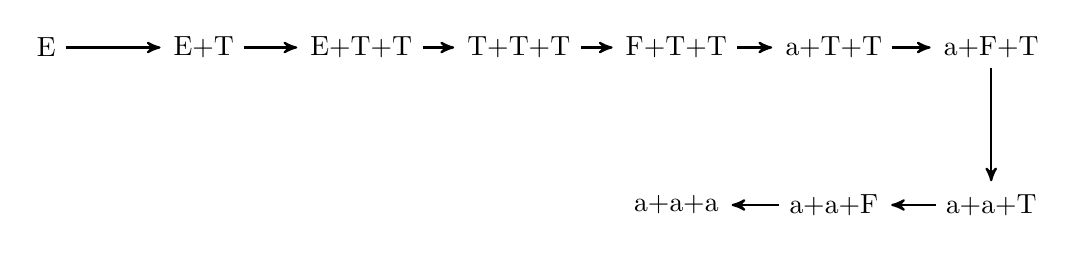
\begin{tikzpicture}[->,>=stealth',shorten >=1pt,auto,node distance=2cm,
  thick,main node/.style={circle,fill=blue!20,draw,font=\sffamily\Large\bfseries}]
  \node[] (1) {E};
  \node[] (2) [right of=1] {E+T};
  \node[] (3) [right of=2] {E+T+T};
  \node[] (4) [right of=3] {T+T+T};
  \node[] (5) [right of=4] {F+T+T};
  \node[] (6) [right of=5] {a+T+T};
  \node[] (7) [right of=6] {a+F+T};
  \node[] (8) [below of=7] {a+a+T};
  \node[] (9) [left of=8] {a+a+F};
  \node[] (10) [left of=9] {a+a+a};
  \path[every node/.style={font=\sffamily\small}]
    (1) edge node {} (2)
    (2) edge node {} (3)
    (3) edge node {} (4)
    (4) edge node {} (5)
    (5) edge node {} (6)
    (6) edge node {} (7)
    (7) edge node {} (8)
    (8) edge node {} (9)
    (9) edge node {} (10);
  \end{tikzpicture}
  \subsection*{(d)}
\subsubsection*{Parse tree}
\begin{tikzpicture}[-,>=stealth',shorten >=1pt,auto,node distance=1cm,
  thick,main node/.style={circle,fill=blue!20,draw,font=\sffamily\Large\bfseries}]
  \node[] (h) {};
  \node[] (1) [right of=h,right of=h,right of=h] {E};
  \node[] (2) [below of=1] {T};
  \node[] (3) [below of=2] {F};
  \node[] (4) [below of=3,left of=3] {(};
  \node[] (5) [below of=3] {E};
  \node[] (6) [below of=3,right of=3] {)};
  \node[] (7) [below of=5] {T};
  \node[] (8) [below of=7] {F};
  \node[] (9) [below of=8,left of=8] {(};
  \node[] (10) [below of=8] {E};
  \node[] (11) [below of=8,right of=8] {)};
  \node[] (12) [below of=10] {T};
  \node[] (13) [below of=12] {F};
  \node[] (14) [below of=13] {a};
  \path[every node/.style={font=\sffamily\small}]
    (1) edge node {} (2)
    (2) edge node {} (3)
    (3) edge [bend right] node {} (4)
    		edge node {} (5)
    		edge[bend left] node {} (6)
    (5) edge node {} (7)
    (7) edge node {} (8)
    (8) edge [bend right] node {} (9)
    		edge node {} (10)
    		edge[bend left] node {} (11)
    	(10) edge node {} (12)
    (12) edge node {} (13)
    	(13) edge node {} (14);
  \end{tikzpicture}
\subsubsection*{Derivation}
  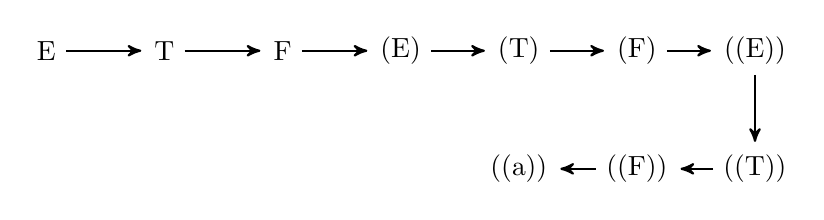
\begin{tikzpicture}[->,>=stealth',shorten >=1pt,auto,node distance=1.5cm,
  thick,main node/.style={circle,fill=blue!20,draw,font=\sffamily\Large\bfseries}]
  \node[] (1) {E};
  \node[] (2) [right of=1] {T};
  \node[] (3) [right of=2] {F};
  \node[] (4) [right of=3] {(E)};
  \node[] (5) [right of=4] {(T)};
  \node[] (6) [right of=5] {(F)};
  \node[] (7) [right of=6] {((E))};
  \node[] (8) [below of=7] {((T))};
  \node[] (9) [left of=8] {((F))};
  \node[] (10) [left of=9] {((a))};
  \path[every node/.style={font=\sffamily\small}]
    (1) edge node {} (2)
    (2) edge node {} (3)
    (3) edge node {} (4)
    (4) edge node {} (5)
    (5) edge node {} (6)
    (6) edge node {} (7)
    (7) edge node {} (8)
    (8) edge node {} (9)
    (9) edge node {} (10);
  \end{tikzpicture}
  \section*{Question 2.2}
  \subsection*{(a)}
  Language A = $\{a^{m}b^{n}c^{n}|m,n \geq 0\}$.
  Language B = $\{a^{n}b^{n}c^{m}|m,n \geq 0\}$.
  The language that is produced by taking the 
  intersection of language A and B is $\{a^{n}b^{n}c^{n}|n \geq 0\}$. Call this new language C.
  To prove that CFL are not closed used under intersection we'll
  assume that C is a CFL then prove by contradiction that C is not and thus proving that CFL in general are not closed under intersection.
  \paragraph*{Proof}
  Let C = $\{a^{n}b^{n}c^{n}|n \geq 0\}$ and let the pumping length be p given by the pumping lemma. Let $s$ be the string $a^{p}b^{p}c^{p}$.
 Divide s up into 5 section $uvxyz$.
 
 If v and y consisted of the same a alphabet element and s $uv^{i}xy^{i}z$ is pumped with $i = 0$ then the string in the from $uxz$ is formed. This string does not contain the same amount of a's, b's and c's which is a contradiction. 
 
 If v and y consisted of different alphabet letters and s is pumped with $i = 0$. Then number of a's, b's and c's will
 not be the same because only two will change and one will remain constant. This causes a contradiction.
 
 If v and y consisted of multiple different alphabet letters and s is pumped with $i = 2$ then the string in the form $uvvxyyx$ is formed. Since v and/or y consists of multiple different different alphabet letters this new string contradicts the original description.

This thus proves that CFL are not closed under intersection.
\subsection*{(b)}
In 2.2.a we proved that CFL are not closed under intersection.
Now we will prove that CFL are not closed under complementation by using DeMorgan's Law ($\overline{A\cup B} = \overline{A}\cap \overline{B}$). DeMorgan's law can be rewritten into the follow form $\overline{\overline{A}\cup \overline{B}} = A\cap B$. Lets assume that A and B are the same as defined in 2.2.a. The right hand side is the intersection of A and B. Since CFL is not closed under intersection the right hand side doesn't hold for 
CFL thus the left hand side also doesn't hold for CFL. Thus CFL are not closed under complementation.
\section*{Question 2.4}
\subsection*{(a)}
\begin{eqnarray}
A &=& 0A|1B\nonumber\\
B &=& 0B|1C\nonumber\\
C &=& 0C|1D\nonumber\\
D &=& 0D|1D|\epsilon\nonumber
\end{eqnarray}
\subsection*{(b)}
\begin{eqnarray}
A &=& 0B0|1B1|1|0\nonumber\\
B &=& 0B|1B|\epsilon\nonumber
\end{eqnarray}
\subsection*{(c)}
\begin{eqnarray}
A &=& 0B|1B\nonumber\\
B &=& 0A|1A|\epsilon\nonumber
\end{eqnarray}
\subsection*{(b)}
\begin{eqnarray}
A &=& BAB|0\nonumber\\
B &=& 0|1\nonumber
\end{eqnarray}
\subsection*{(e)}
\begin{eqnarray}
A &=& 1A1|0A0|\epsilon\nonumber
\end{eqnarray}
\subsection*{(f)}
\begin{eqnarray}
A &=& A\nonumber
\end{eqnarray}
\section*{Question 2.12}
\section*{Question 2.14}
\subsection*{Step 1}
\begin{eqnarray}
S$_{0}$ &=& A\nonumber\\
A &=& BAB|B|\epsilon\nonumber\\
B &=& 00|\epsilon\nonumber
\end{eqnarray}
\subsection*{Step 2}
\begin{eqnarray}
S$_{0}$ &=& A\nonumber\\
A &=& BAB|AB|BA|B|\epsilon\nonumber\\
B &=& 00\nonumber
\end{eqnarray}
\subsection*{Step 3}
\begin{eqnarray}
S$_{0}$ &=& BAB|AB|BA|B|\epsilon\nonumber\\
A &=& BAB|AB|BA|B|\epsilon\nonumber\\
B &=& 00\nonumber
\end{eqnarray}
\subsection*{Step 4}
\begin{eqnarray}
S$_{0}$ &=& BAB|AB|BA|00|\epsilon\nonumber\\
A &=& BAB|AB|BA|00|\epsilon\nonumber\\
B &=& 00\nonumber
\end{eqnarray}
\subsection*{Step 5}
\begin{eqnarray}
S$_{0}$ &=& BB_{1}|AB|BA|00|\epsilon\nonumber\\
A &=& BB_{1}|AB|BA|00|\epsilon\nonumber\\
B &=& 00\nonumber\\
B_{1} &=& AB\nonumber
\end{eqnarray}
\section*{Question 2.27}
\subsection*{(a)}
For a grammar to be ambiguous it needs to have atleast two left most derivations for a string w. The given grammer has atleast two left most derivations for the string ``if condition then if condition then a:=1 else a:=1''. Note \texttt{itc = if condition then}. 
\subsubsection*{Derivation 1}
  \begin{tikzpicture}[->,>=stealth',shorten >=1pt,auto,node distance=1.5cm,
  thick,main node/.style={circle,fill=blue!20,draw,font=\sffamily\Large\bfseries}]
  \node[] (n) {};
  \node[] (1) [right of=n,right of=n,right of=n]{STMT};
  \node[] (2) [below of=1] {IF-THEN};
  \node[] (3) [below of=1, left of=2] {ict};
  \node[] (4) [below of=1,right of=2] {STMT};
  \node[] (5) [below of=4] {IF-THEN-ELSE};
  \node[] (6) [right of=5] {(F)};
  \node[] (7) [right of=6] {((E))};
  \node[] (8) [below of=7] {((T))};
  \node[] (9) [left of=8] {((F))};
  \node[] (10) [left of=9] {((a))};
  \path[every node/.style={font=\sffamily\small}]
    (1) edge node {} (2)
    (2) edge node {} (3)
        edge node {} (4)
    (4) edge node {} (5)
    (5) edge node {} (6)
    (6) edge node {} (7)
    (7) edge node {} (8)
    (8) edge node {} (9)
    (9) edge node {} (10);
  \end{tikzpicture}
\subsubsection*{Derivation 2}
\end{document}